\documentclass{beamer}
\usepackage[UTF8,space,hyperref]{ctex}
\usepackage{color}
\usepackage{graphicx} % ⋯⋯导言区其他内容
\usepackage{amsmath}

\usetheme{Luebeck}
\author{A Large-Scale Study on Regularization and Normalization in GANs}
\title{GAN中的正则化和归一化研究}


\begin{document}
 
\frame{\titlepage}

\begin{frame}[c]\frametitle{GAN训练}
\begin{itemize}
    \item 存在训练深度神经网络相关的优化问题
    \item GAN的训练还对下面几种选择非常敏感:
    \begin{itemize}
        \item 损失函数
        \item 网络结构
        \item 正则化和归一化s
    \end{itemize}

\end{itemize}
\end{frame}

\begin{frame}[c]\frametitle{GAN}
    \begin{itemize}
       \item 论文对这些方法进行了全面的实验分析,通过超参数优化,在几个流行的大规模数据集上进行实验。
       \item 超参数集还参考了一些文献中提出的“好”的超参数集, 以及通过贝叶斯优化获得的参数集。
    \end{itemize}
\end{frame}

\begin{frame}[c]\frametitle{一些概念}
    \begin{itemize}
        \item {\color{red}消融研究( Ablation study )}:
        指通过移除某个模型或者算法的某些特征,来观察这些特征对模型效果的影响。
    \end{itemize}
\end{frame}

\begin{frame}[c]\frametitle{生成器和判别器的结构}
    \begin{itemize}
        \item DC-GAN
        \item ResNet: 
        \begin{itemize}
            \item 生成器中有5个ResNet块,在判别器中有6个ResNet块。
        \end{itemize}
        \item 都使用Adam优化器训练。
    \end{itemize}
\end{frame}

\begin{frame}[c]\frametitle{评估准则(IS)}
    \begin{itemize}
        \item Inception Score(IS)
        $$IS(G) = exp(\mathbb{E}_{x\backsim p_g}D_{KL}(p(y|x)||p(y)))$$
        其中:\newline
        exp:仅仅是为了好看,没有具体含义。\newline
        $x\backsim P_g$ :表示从生成器中生图片。\newline
        $p(y|x)$: 判别器输出x的概率的分布  \newline
        $p_y$: N 个生成的图片,各自得到一个自己的概率分布向量,把这些向量求一个平均,得到生成器生成的图片全体在所有类别上的边缘分布
    \end{itemize}
\end{frame}

\begin{frame}[c]\frametitle{评估准则(FID)}
    \begin{itemize}
        \item FID
        $$FID =  \left \| \mu_x - \mu_y \right \|_2^2 + Tr(\Sigma_x + \Sigma_y - 2(\Sigma_x\Sigma_y)^\frac{1}{2}{})$$
        其中(μx,Σx)和(μy,Σy)分别是来自P和Q的嵌入样本的均值和协方差。作者认为,FID与人类的判断相一致,并且比IS更加稳健。
    \end{itemize}
\end{frame}

\begin{frame}[c]\frametitle{数据集}
    \begin{itemize}
        \item CIFAR10
        \begin{itemize}
            \item 60K个训练图像和10K个测试图像
        \end{itemize}
        \item CELEBA-HQ-128
        \begin{itemize}
            \item 30K张图像,3K个作为测试集
        \end{itemize}
        \item LSUN-BEDROOM
        \begin{itemize}
            \item 300万张图像, 其中30588张作为测试集
        \end{itemize}
    \end{itemize}
\end{frame}

\begin{frame}[c]\frametitle{结论}
    \begin{itemize}
        \item 证明梯度惩罚以及谱归一化适用于复杂的网络结构
        \item 通过分析损失函数的影响,非饱和损失在数据集和超参数之间是足够稳定的
        \item 实验表明类似的结论适用于最新模型
        \item 当计算资源有限时,应将非饱和GAN损失和谱归一化视为将GAN应用于新数据集时的默认选择。 
                给定额外的计算资源,建议添加Gulrajani等人的梯度惩罚。
    \end{itemize}
\end{frame}

\begin{frame}[c]\frametitle{正则化和归一化}
    \begin{itemize}
        \item 主要比较了下面几种归一化和正则化方法:
        \begin{itemize}
            \item 批量归一化(BN)、层归一化(LN) 、谱归一化(SN)
            \item 梯度惩罚(GP) 、 Dragan惩罚(DR) 、 L2正则化
        \end{itemize}
        \item 实验时设置损失为非饱和损失。
    \end{itemize}
\end{frame}

\begin{frame}[c]\frametitle{正则化和归一化(网络结构的选择)}
    \begin{figure}[h]
        \begin{minipage}[t]{0.4\linewidth}%并排放两张图片,每张占行的0.4,下同 
        \centering     %插入的图片居中表示
        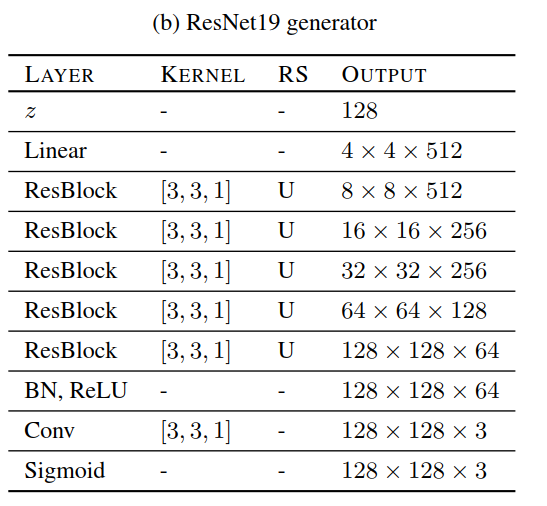
\includegraphics[width=1.2\textwidth]{G.png}
        \caption{生成器结构.}%图片的名称
        \end{minipage} 
        \hfill
        \begin{minipage}[t]{0.4\linewidth}
        \centering
        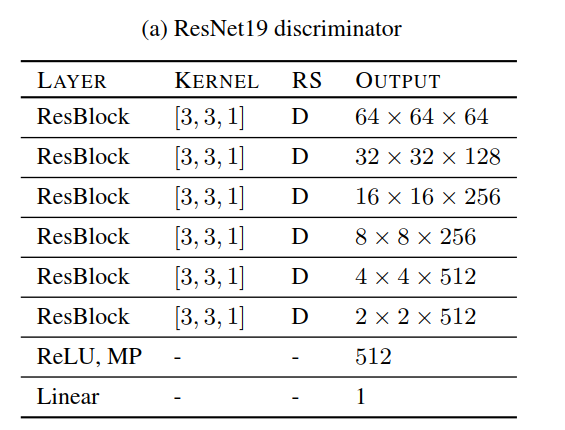
\includegraphics[width=1.2\textwidth]{D.png}
        \caption{判别器结构.}%图片的名称
        \end{minipage}
    \end{figure}
\end{frame}

\begin{frame}[c]\frametitle{正则化和归一化(超参数选择)}
    \begin{figure}[h]
        \begin{minipage}[t]{0.4\linewidth}%并排放两张图片,每张占行的0.4,下同 
        \centering     %插入的图片居中表示
        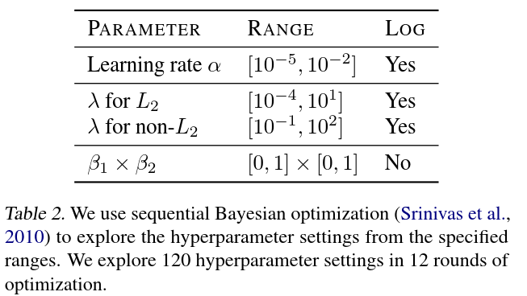
\includegraphics[width=1.2\textwidth]{hyperParmetersWithBayes.png}
        \caption{贝叶斯优化设置.}%图片的名称
        \end{minipage} 
        \hfill
        \begin{minipage}[t]{0.4\linewidth}
        \centering
        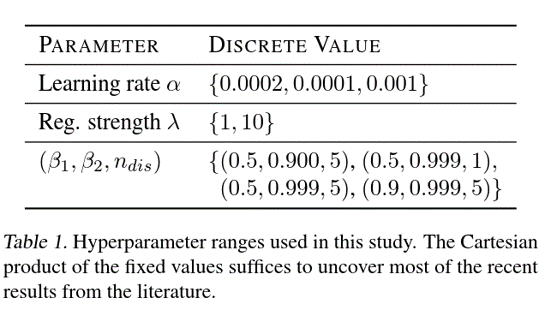
\includegraphics[width=1.2\textwidth]{hyperParmetersWithLiterature.png}
        \caption{根据文献选择的.}%图片的名称
        \end{minipage}
    \end{figure}
\end{frame}

\begin{frame}[c]\frametitle{正则化和归一化(结果)}
    \begin{figure}[ht]
        \centering
        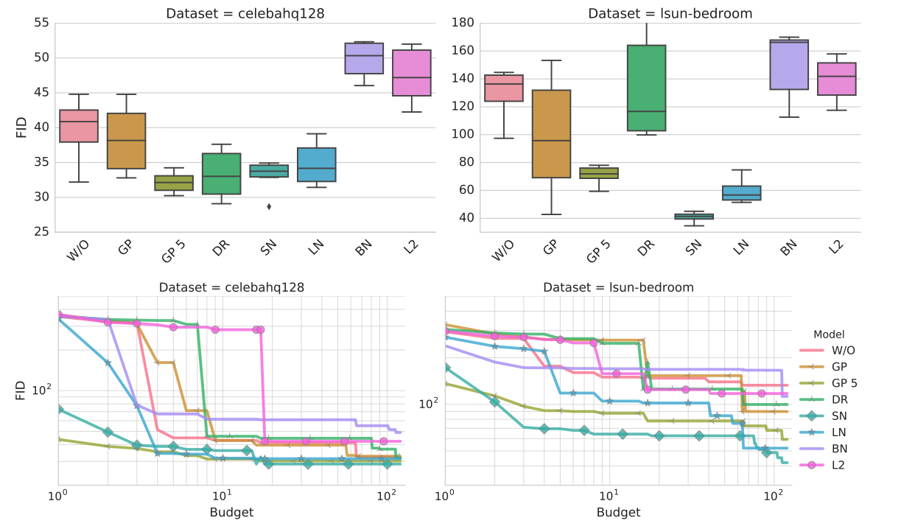
\includegraphics[scale=0.5]{result1.png}  %这个是图片的绝对路径
        \caption{top 5\% model}
    \end{figure}
\end{frame}

\begin{frame}[c]\frametitle{正则化和归一化(结论)}
    \begin{itemize}
        \item 向判别器添加批量归一化会降低性能
        \item 梯度惩罚(GP)可以帮助降低FID,但它不能稳定训练
        \item 谱归一化有助于提高模型质量,比梯度惩罚具有更高的计算效率
        \item GP惩罚的模型可能受益于判别器与生成器更新比例为5:1
        \item 在一项单独的消融研究中,运行额外的10万步优化程序可能会提高GP惩罚模型的性能
    \end{itemize}
\end{frame}

\begin{frame}[c]\frametitle{损失函数}
    研究损失函数的变化是否也能得到上述的结论?
\end{frame}

\begin{frame}[c]\frametitle{损失函数}
    \begin{figure}[top]
        \centering
        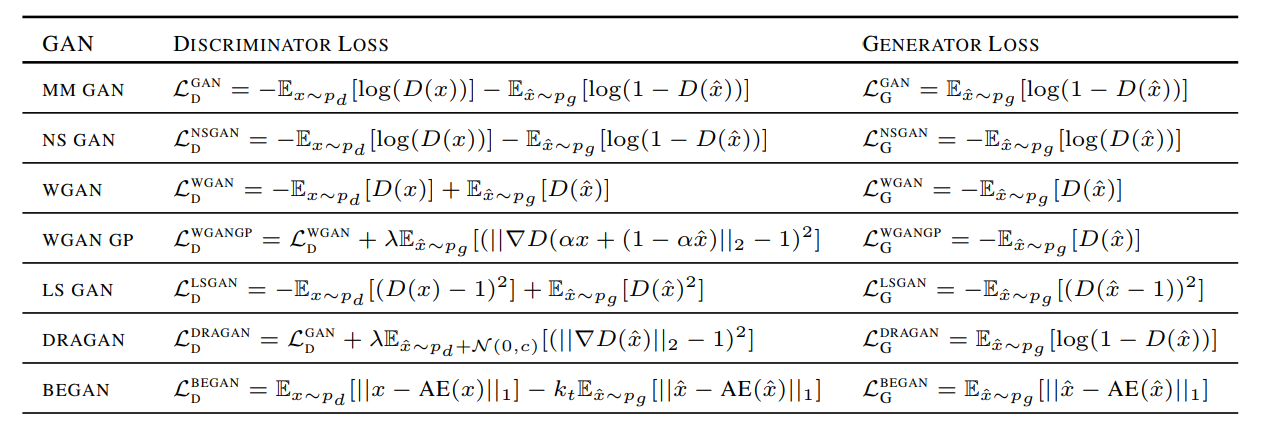
\includegraphics[scale=0.3]{loss.png}  %这个是图片的绝对路径
        \caption{GAN的损失函数}
    \end{figure}
\end{frame}

\begin{frame}[c]\frametitle{损失函数}
    \begin{itemize}
        \item 非饱和损失(NS)
$$\mathcal{L}_D^{NSGAN} = -\mathbb{E}_{x\backsim p_d}[log(D(x))] - \mathbb{E}_{\hat{x}\backsim p_g}[log(1 - D(\hat{x}))] $$
$$\mathcal{L}_G^{NSGAN} = \mathbb{E}_{\hat{x}\backsim p_g}[log(1 - D(\hat{x}))]$$
        \item 最小二乘损失(LS) 
$$\mathcal{L}_D^{LSGAN} = -\mathbb{E}_{x\backsim p_d}[log(D(x) - 1)^2] + \mathbb{E}_{\hat{x}\backsim p_g}[log(D(\hat{x}))]$$
$$\mathcal{L}_G^{LSGAN} = -\mathbb{E}_{\hat{x}\backsim p_g}[log(D(\hat{x}) - 1)^2]$$
        \item Wasserstein loss
       
    \end{itemize}
\end{frame}

\begin{frame}[c]\frametitle{损失函数(结果)}
    \begin{figure}[top]
        \centering
        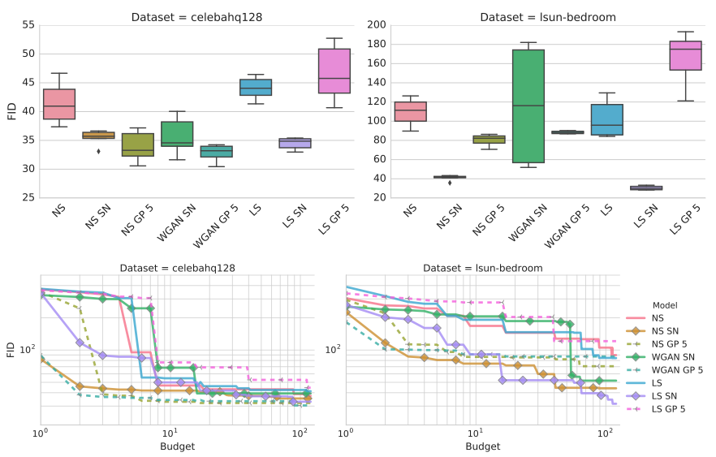
\includegraphics[scale=0.5]{lossResult.png}
        \caption{top 5\% model损失函数的影响}
    \end{figure}
\end{frame}

\begin{frame}[c]\frametitle{损失函数(结论)}
    \begin{itemize}
        \item 谱归一化提高了两个数据集的模型质量
        \item 梯度惩罚也会对模型的性能提升有所帮助
        \item 原始GAN的非饱和损失跟其它改进的损失结果差距不大
    \end{itemize}
\end{frame}

\begin{frame}[c]\frametitle{网络结构}
    考虑上述的结果是否也适用于不同的网络结构,为此还对SNDCGAN进行了研究。主要考虑下面几项:
    \begin{itemize}
        \item 非饱和GAN损失
        \item 梯度惩罚
        \item 谱归一化
    \end{itemize}
\end{frame}

\begin{frame}[c]\frametitle{网络结构的消融研究}
    作者注意到与目前github的实现相比,
    Resnet架构有六个细微差别。进行了消融研究以验证这些差异的影响。详细描述如下:
    \begin{enumerate}
        \item[1] 默认情况:ResNet CIFAR架构,具有谱归一化和非饱和GAN损失
        \item[2] 残差连接:使用输入作为判别器ResBlock中残差连接的输出。 默认情况下,它是一个带有3x3内核的卷积层。
        \item[3] CIN: 使用$c_i$作为判别器ResBlock隐藏层输出通道数目。默认情况下设置为$c_o$, 但是MiyatoMiyatoet al. (2018)使用$c_o$作为第一层的输出通道数,其余的通道数设置为$c_i$
    \end{enumerate}
\end{frame}

\begin{frame}[c]\frametitle{网络结构的消融研究}
    \begin{enumerate}
        \item[4] OPT: 判别器的第一个残差块设置一些优化,包括:
        (1)没有Relu激活
        (2)一个包含残差连接的卷积层
        (3)在残差块儿内部,用$c_o$替代$c_i$.
        \item[5] CIN OPT: 将CIN和OPT的设置结合
        \item[6] 判别器输出层使用reduce sum操作, 默认使用reduce mean
    \end{enumerate}
    结果如下图所示。
\end{frame}


\begin{frame}[c]\frametitle{网络结构的消融研究}
    \begin{enumerate}
        \item[7] TAN: 使用Tanh作为生成器输出层激活,判别器输入值的范围为[-1, 1]。默认使用sigmoid激活,判别器输入范围为[0, 1]
        \item[8] EPS: 生成器中BN层使用较大的epsilon:2e-5。TensorFlow默认为1e-5
        \item[9] ALL:将上述的设置综合使用
    \end{enumerate}
\end{frame}


\begin{frame}[c]\frametitle{网络结构的消融研究}
    \begin{figure}[top]
        \centering
        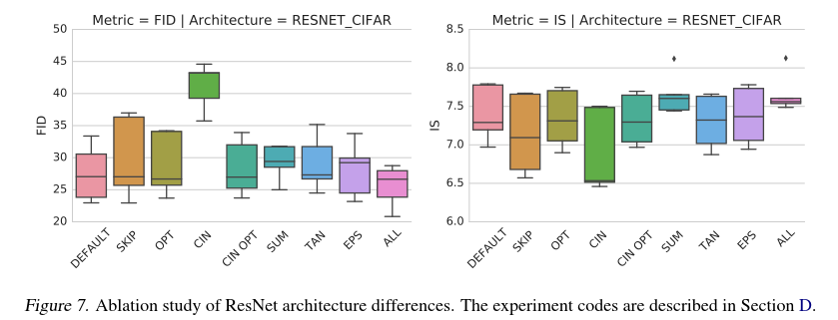
\includegraphics[scale=0.5]{result7.png} 
        \caption{ResNet结构消融结果}
    \end{figure}
    CIN的设置得到的分数最差.当CIN和OPT结合效果有所提升(与其它结果相当),
    根据对CIFAR10结果研究,这些差异的影响很小。
\end{frame}

\begin{frame}[c]\frametitle{一些建议}
    实验中比较普遍的结果是,判别器的Lipschitzc常数对模型的性能至关重要,同时进行正则化和归一化可以提高模型的质量。
    为了量化这种效果,将损失固定为非饱和损失,使用Resnet19体系结构,结合几种标准化和正则化方案,使用上面表中所示的超参数设置和随机选择的24个参数。
\end{frame}

\begin{frame}[c]\frametitle{结果}
    \begin{figure}[top]
        \centering
        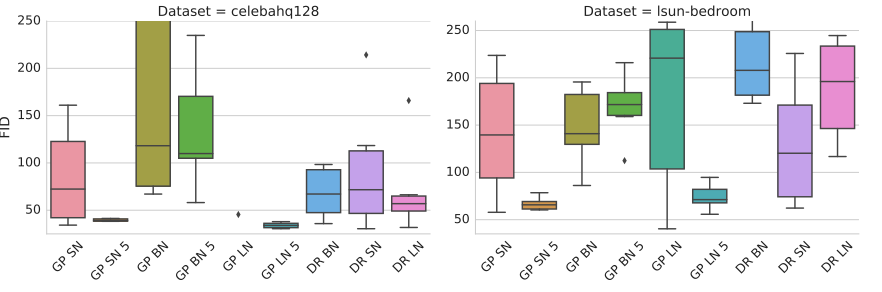
\includegraphics[scale=0.5]{result4.png} 
        \caption{top 5\% model 正则化和归一化结合使用}
    \end{figure}
    可以看出梯度惩罚和SN或LN结合能够很好的提升模型的性能.
\end{frame}

\begin{frame}[c]\frametitle{问题1(不懂)}
    产生上述结果的原因:
    \color{red} Gradient penalty coupled with spectral normaliza-
    tion (SN) or layer normalization (LN) strongly improves the performance over the baseline. This can be partially explained by the fact
    that SN doesn’t ensure that the discriminator is 1-Lipschitz due to the way convolutional layers are normalized.
\end{frame}

\begin{frame}[c]\frametitle{实验的一些细节}
    \begin{itemize}
        \item 应该根据测试数据集计算FID
        \item 网络结构的详细设计
        \item 数据集的预处理(如放大、裁剪的精确算法)
    \end{itemize}
\end{frame}

\begin{frame}[c]\frametitle{目前存在的一些问题(非确定性)}
    \begin{itemize}
        \item 论文中提出的算法与开源的代码实现不匹配
        \item 良好的算法实现与不良的代码实现之间有着巨大差距
        \item 训练的随机性,即训练相同的模型两次能否获得相同的分数是十分重要的,
        由于某些GPU操作存在随机性,如果禁用这些操作就会造成时间的损失
    \end{itemize}
\end{frame}

\begin{frame}[c]\frametitle{归一化公式}
    \begin{itemize}
        \item 批量归一化
        $$\hat{x^{(k)}} = \frac{x^{(k)} - E[x^{(k)}]}{\sqrt{Var[x^{(k)}]}}$$
        $$y^{(k)} = \gamma^{(k)}\hat{x}^{(k)} + \beta^{(k)}$$
        \item 谱归一化: 可以使网络满足利普西茨约束
        \item 求某一层权值矩阵W的最大特征值$\sigma(W)$
        $$\sigma(W)\simeq\hat{u}W^T\hat{v}$$
        $$W\gets\frac{W}{\sigma(W)}$$
        其中:$\hat{u}$和$\hat{v}$对应矩阵W的特征分解矩阵
        
    \end{itemize}
\end{frame}

\begin{frame}[c]\frametitle{正则化公式}
    \begin{itemize}
        \item 梯度裁剪
        \item  
        \begin{itemize}
                设定裁剪阈值c,损失对参数W的梯度为g, 如果$\left\|g\right\|^2_2 > c$:
                $$g = \frac{c}{\left\| g\right\|_2}\cdot g$$
                否则g保持不变
        \end{itemize}
        \item L2正则化
            $$loss + \left\|\theta\right\|_2$$ 
    \end{itemize}
\end{frame}

\end{document}


